\documentclass[conference]{IEEEtran}

\usepackage{amsmath,amssymb,amsfonts}
\usepackage{graphicx}
\usepackage{booktabs}
\usepackage{cite}
\usepackage{url}
\usepackage{hyperref}

\title{Adaptive Lag-Selective Shrinkage for Robust Coarray MUSIC in Weight-Constrained Sparse Arrays}

\author{
\IEEEauthorblockN{Hossein Molhem}
\IEEEauthorblockA{
Department of Electrical and Computer Engineering\\
Kennesaw State University\\
Email: hmolhem@students.kennesaw.edu}
}

\begin{document}

\maketitle

\begin{abstract}
Weight-constrained sparse arrays reduce mutual-coupling sensitivity by suppressing or eliminating closely spaced sensor-pair contributions. However, the same sparse coarray-weight structure can produce high-variance lag estimates in finite-snapshot regimes. This paper evaluates Adaptive Lag-Selective Shrinkage (ALSS), a post-geometry coarray-domain regularization method applied before virtual covariance reconstruction and Coarray MUSIC processing. A controlled Scenario 3 experiment is performed for the Z5 sparse array using 1000 Monte Carlo trials, ALSS mode \texttt{ar1}, shrinkage parameter $\tau=0.25$, and protected core lag $L_c=3$. Results show that ALSS improves RMSE in 15 of 16 reported conditions, with a mean improvement of approximately $9.85\%$ over reported rows and $9.76\%$ over unique conditions. The improvement is stronger under mutual coupling, where the mean improvement is approximately $13.92\%$, compared with $5.60\%$ in the no-coupling case. These results support ALSS as a useful statistical denoising layer for the Z5 geometry under the tested Scenario 3 conditions, while motivating broader validation across additional sparse-array geometries.
\end{abstract}

\begin{IEEEkeywords}
Direction-of-arrival estimation, sparse arrays, coarray MUSIC, mutual coupling, adaptive shrinkage, finite snapshots, weight-constrained sparse arrays.
\end{IEEEkeywords}

\section{Introduction}

Sparse sensor arrays are widely used in direction-of-arrival (DOA) estimation because they can synthesize a virtual aperture through difference-coarray processing while using fewer physical sensors than a fully populated uniform linear array~\cite{pal2010nested,vaidyanathan2011coprime,pal2011coprimeMusic}. This virtual-aperture advantage is especially useful in subspace-based methods such as MUSIC, where additional coarray degrees of freedom can improve source resolvability when the required statistical assumptions are satisfied~\cite{schmidt1986music,vantrees2002optimum}.

In practical arrays, however, mutual coupling can distort the received spatial data and degrade DOA estimation accuracy. Weight-constrained sparse arrays address this issue at the geometry level by suppressing or eliminating sensor-pair contributions at critical small lags, such as $w(1)=0$ or $w(1)=w(2)=0$~\cite{kulkarni2024wcsa}. The Z5 geometry considered in this paper follows this design philosophy: it reduces the most coupling-sensitive short-spacing contributions while preserving a useful one-sided coarray segment for Coarray MUSIC processing.

Geometry alone does not remove all estimation error. In finite-snapshot regimes, the sample covariance matrix is noisy, and the resulting coarray lag estimates do not have equal reliability. A lag with a small coarray weight $w[\ell]$ is estimated from fewer physical covariance entries than a high-weight lag. Therefore, even when the geometry is favorable for mutual-coupling robustness, low-weight and long-lag estimates may inject variance into the virtual covariance matrix used by Coarray MUSIC.

This paper evaluates Adaptive Lag-Selective Shrinkage (ALSS) as a post-geometry statistical denoising layer for this problem. ALSS is applied after sample covariance estimation and coarray lag averaging, but before virtual covariance reconstruction. It does not change the physical Z5 sensor geometry or the antenna coupling mechanism. Instead, it regularizes the estimated coarray correlations so that low-confidence lags have reduced influence on the reconstructed virtual covariance matrix.

The goal of this paper is deliberately focused. We do not claim universal ALSS optimality across all sparse arrays or all operating regimes. Instead, we test whether a fixed ALSS configuration provides stable RMSE improvement for the Z5 array under Scenario 3 conditions with and without mutual coupling.

The main contributions are:
\begin{itemize}
    \item A focused evaluation of ALSS as a post-geometry coarray-domain denoising layer for the Z5 sparse array.
    \item A 1000-trial Scenario 3 validation using fixed ALSS parameters: \texttt{ar1}, $\tau=0.25$, and $L_c=3$.
    \item A coupling-aware comparison showing that ALSS gives stronger average RMSE improvement under mutual coupling than under no-coupling conditions.
    \item A compact conference-paper result set connecting Z5 coarray geometry, finite-snapshot lag variance, representative MUSIC spectra, and trial-1000 RMSE trends.
\end{itemize}

\section{Background}

\subsection{Coarray MUSIC}

For an $N$-sensor array with sensor locations $\{n_i\}_{i=1}^{N}$, the narrowband received signal can be written using the standard narrowband array-processing model~\cite{vantrees2002optimum} as
\begin{equation}
    \mathbf{x}[k] = \mathbf{A}(\boldsymbol{\theta})\mathbf{s}[k] + \mathbf{n}[k],
\end{equation}
where $\mathbf{A}(\boldsymbol{\theta})$ is the array manifold matrix, $\mathbf{s}[k]$ is the source vector, and $\mathbf{n}[k]$ is additive noise.

The sample covariance matrix is estimated as
\begin{equation}
    \hat{\mathbf{R}}_x =
    \frac{1}{M}
    \sum_{k=1}^{M}
    \mathbf{x}[k]\mathbf{x}^{H}[k],
\end{equation}
where $M$ is the number of snapshots.

The difference coarray is the set of all pairwise sensor-position differences,
\begin{equation}
    \mathcal{D} = \{n_i - n_j: i,j = 1,\ldots,N\}.
\end{equation}
For each lag $\ell$, the coarray weight $w[\ell]$ is the number of sensor pairs that produce that lag. A lag-domain covariance estimate can be obtained by averaging all covariance entries associated with the same lag:
\begin{equation}
    \hat{r}[\ell] =
    \frac{1}{w[\ell]}
    \sum_{n_i-n_j=\ell}
    [\hat{\mathbf{R}}_x]_{i,j}.
\end{equation}

The lag sequence is then used to form a virtual Toeplitz covariance matrix for Coarray MUSIC, which builds on the subspace principle of the MUSIC algorithm~\cite{schmidt1986music}.

\subsection{Finite-Snapshot Variance Issue}

In finite-snapshot regimes, the reliability of $\hat{r}[\ell]$ depends on both the number of snapshots and the number of sensor-pair averages available for lag $\ell$. A useful first-order variance proxy is
\begin{equation}
    \widehat{V}[\ell] \propto \frac{\hat{\sigma}_n^2}{w[\ell]M}.
\end{equation}
Thus, lags with small $w[\ell]$ and limited $M$ may have larger estimation variance. This motivates a lag-selective regularization method that protects reliable core lags while reducing the influence of noisy low-confidence lags.

\section{Adaptive Lag-Selective Shrinkage}

ALSS is a coarray-domain regularization step applied after sample covariance estimation and lag averaging, but before virtual covariance reconstruction. The processing chain is
\begin{equation}
    \mathbf{X}
    \rightarrow
    \hat{\mathbf{R}}_x
    \rightarrow
    \hat{r}[\ell]
    \rightarrow
    \hat{r}_{\mathrm{ALSS}}[\ell]
    \rightarrow
    \hat{\mathbf{R}}_v
    \rightarrow
    \text{Coarray MUSIC}.
\end{equation}
Thus, ALSS does not modify the physical sensor geometry, the antenna pattern, or the mutual-coupling mechanism itself. It only modifies the estimated coarray correlations used to construct the virtual covariance matrix.

The motivation is that not all lag estimates have equal confidence. For lag $\ell$, the empirical correlation $\hat{r}[\ell]$ is obtained by averaging $w[\ell]$ physical covariance entries. A low-weight lag has fewer sensor-pair contributions and is therefore more sensitive to finite-snapshot noise. ALSS uses this observation to shrink low-confidence lag estimates while protecting the most reliable core lags.

The implemented ALSS form used in this paper is
\begin{equation}
    \hat{r}_{\mathrm{ALSS}}[\ell]
    =
    \left(1-\alpha[\ell]\right)\hat{r}[\ell]
    +
    \alpha[\ell] r_{\mathrm{prior}}[\ell],
\end{equation}
where $\alpha[\ell]\in[0,1]$ is the shrinkage weight. A larger value of $\alpha[\ell]$ moves the lag estimate more strongly toward the prior. For the AR(1) mode used in this experiment, the prior is fitted from protected low-lag correlations and then extrapolated to less reliable lags. The shrinkage weight is scheduled using a variance proxy of the form
\begin{equation}
    \widehat{V}[\ell]
    =
    \frac{\hat{\sigma}^{2}}{M w[\ell]},
\end{equation}
where $M$ is the number of snapshots and $w[\ell]$ is the coarray weight.

The AR(1)-mode shrinkage weight used by the implementation can be summarized as
\begin{equation}
    \alpha[\ell]
    =
    \frac{\widehat{V}[\ell]}
    {\widehat{V}[\ell]
    +
    \tau
    \left|
        \hat{r}[\ell]-r_{\mathrm{prior}}[\ell]
    \right|^2
    +
    \epsilon},
\end{equation}
where $\tau$ controls the shrinkage strength and $\epsilon$ is a small numerical-stability constant. In this convention, $\alpha[\ell]$ is not a retention factor; it is the amount of movement toward the prior.

In the reported experiment, the selected ALSS configuration is
\begin{equation}
    \text{mode}=\texttt{ar1}, \qquad \tau=0.25, \qquad L_c=3.
\end{equation}
Core lags $0\leq \ell \leq L_c$ are protected from shrinkage. After shrinkage, Hermitian symmetry is enforced so that
\begin{equation}
    \hat{r}_{\mathrm{ALSS}}[-\ell]
    =
    \hat{r}^{*}_{\mathrm{ALSS}}[\ell],
\end{equation}
which preserves the structure required for virtual covariance reconstruction and Coarray MUSIC processing.

\section{Experimental Setup}

\subsection{Scenario and Array}

This paper evaluates Scenario 3 for the canonical Z5 sparse array. The physical sensor locations, expressed on the half-wavelength grid, are
\begin{equation}
    \mathbf{z}_{5} = [0,\;5,\;8,\;11,\;14,\;17,\;21].
\end{equation}
The trial-1000 result is treated as the primary paper-facing validation result. The earlier trial-500 result is retained only as intermediate validation history and is not used as the main quantitative evidence in this paper.

The Z5 sparse array used in this study is shown in Fig.~\ref{fig:z5_geometry}.
Its difference-coarray weight distribution is shown in Fig.~\ref{fig:z5_coarray_weights}.
The geometry suppresses the most coupling-sensitive small lags, with $w(1)=0$ and $w(2)=0$, while retaining nonzero weights at later lags. This structure is useful for reducing short-spacing coupling sensitivity, but it also creates an uneven coarray-weight profile. The uneven lag support motivates the use of ALSS as a post-geometry coarray-domain regularization method.

\begin{figure}[t]
\centering
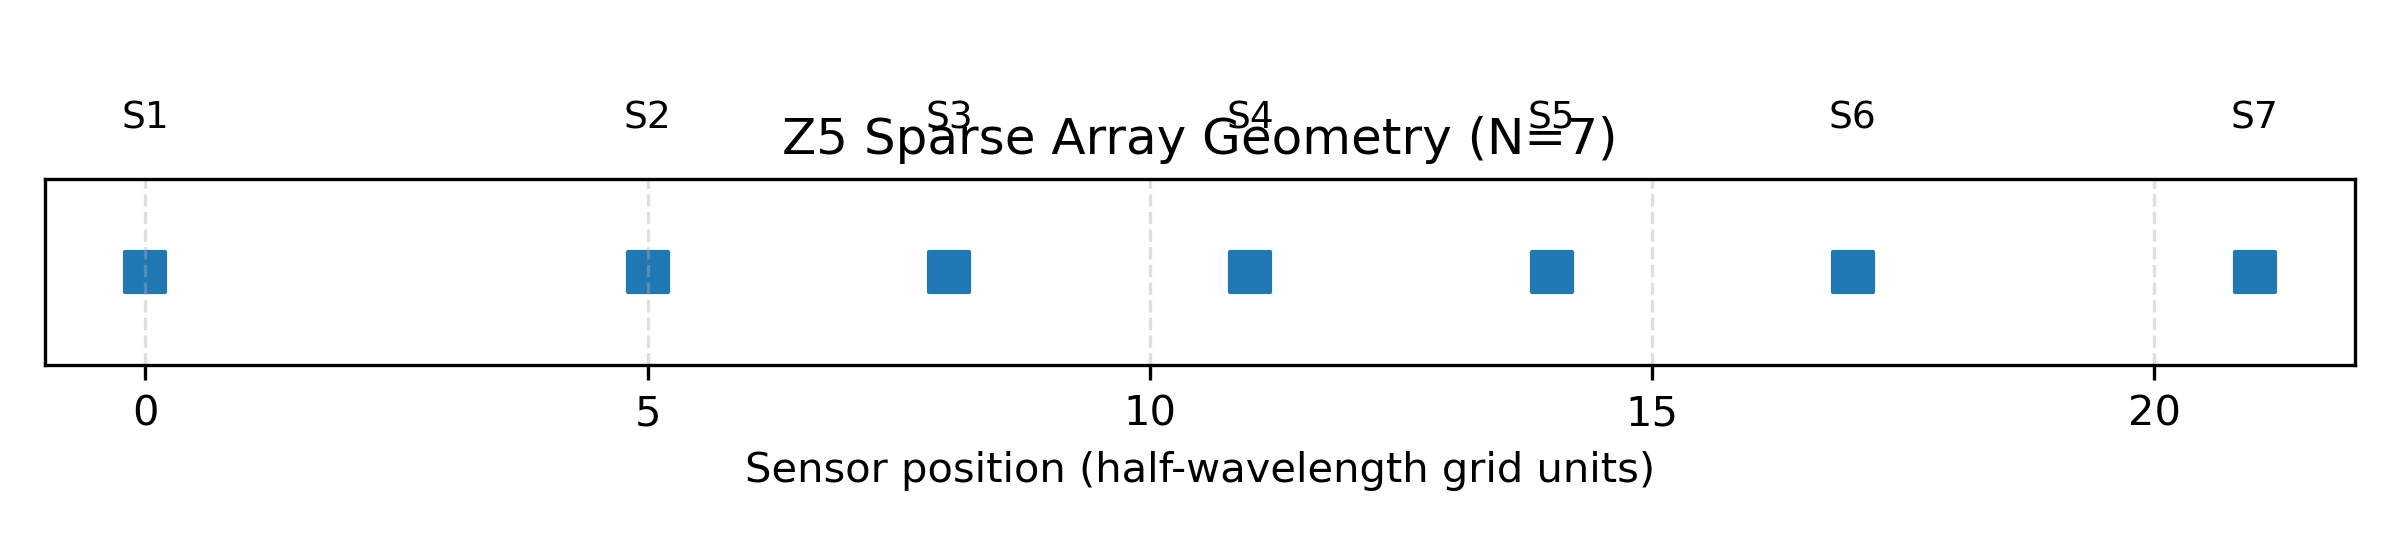
\includegraphics[width=\linewidth]{../../results/figures/paper1_conceptual/z5_sensor_geometry.png}
\caption{Canonical Z5 sparse-array geometry used in the Scenario 3 trial-1000 experiment. Sensor positions are shown on the half-wavelength grid.}
\label{fig:z5_geometry}
\end{figure}

\begin{figure}[t]
\centering
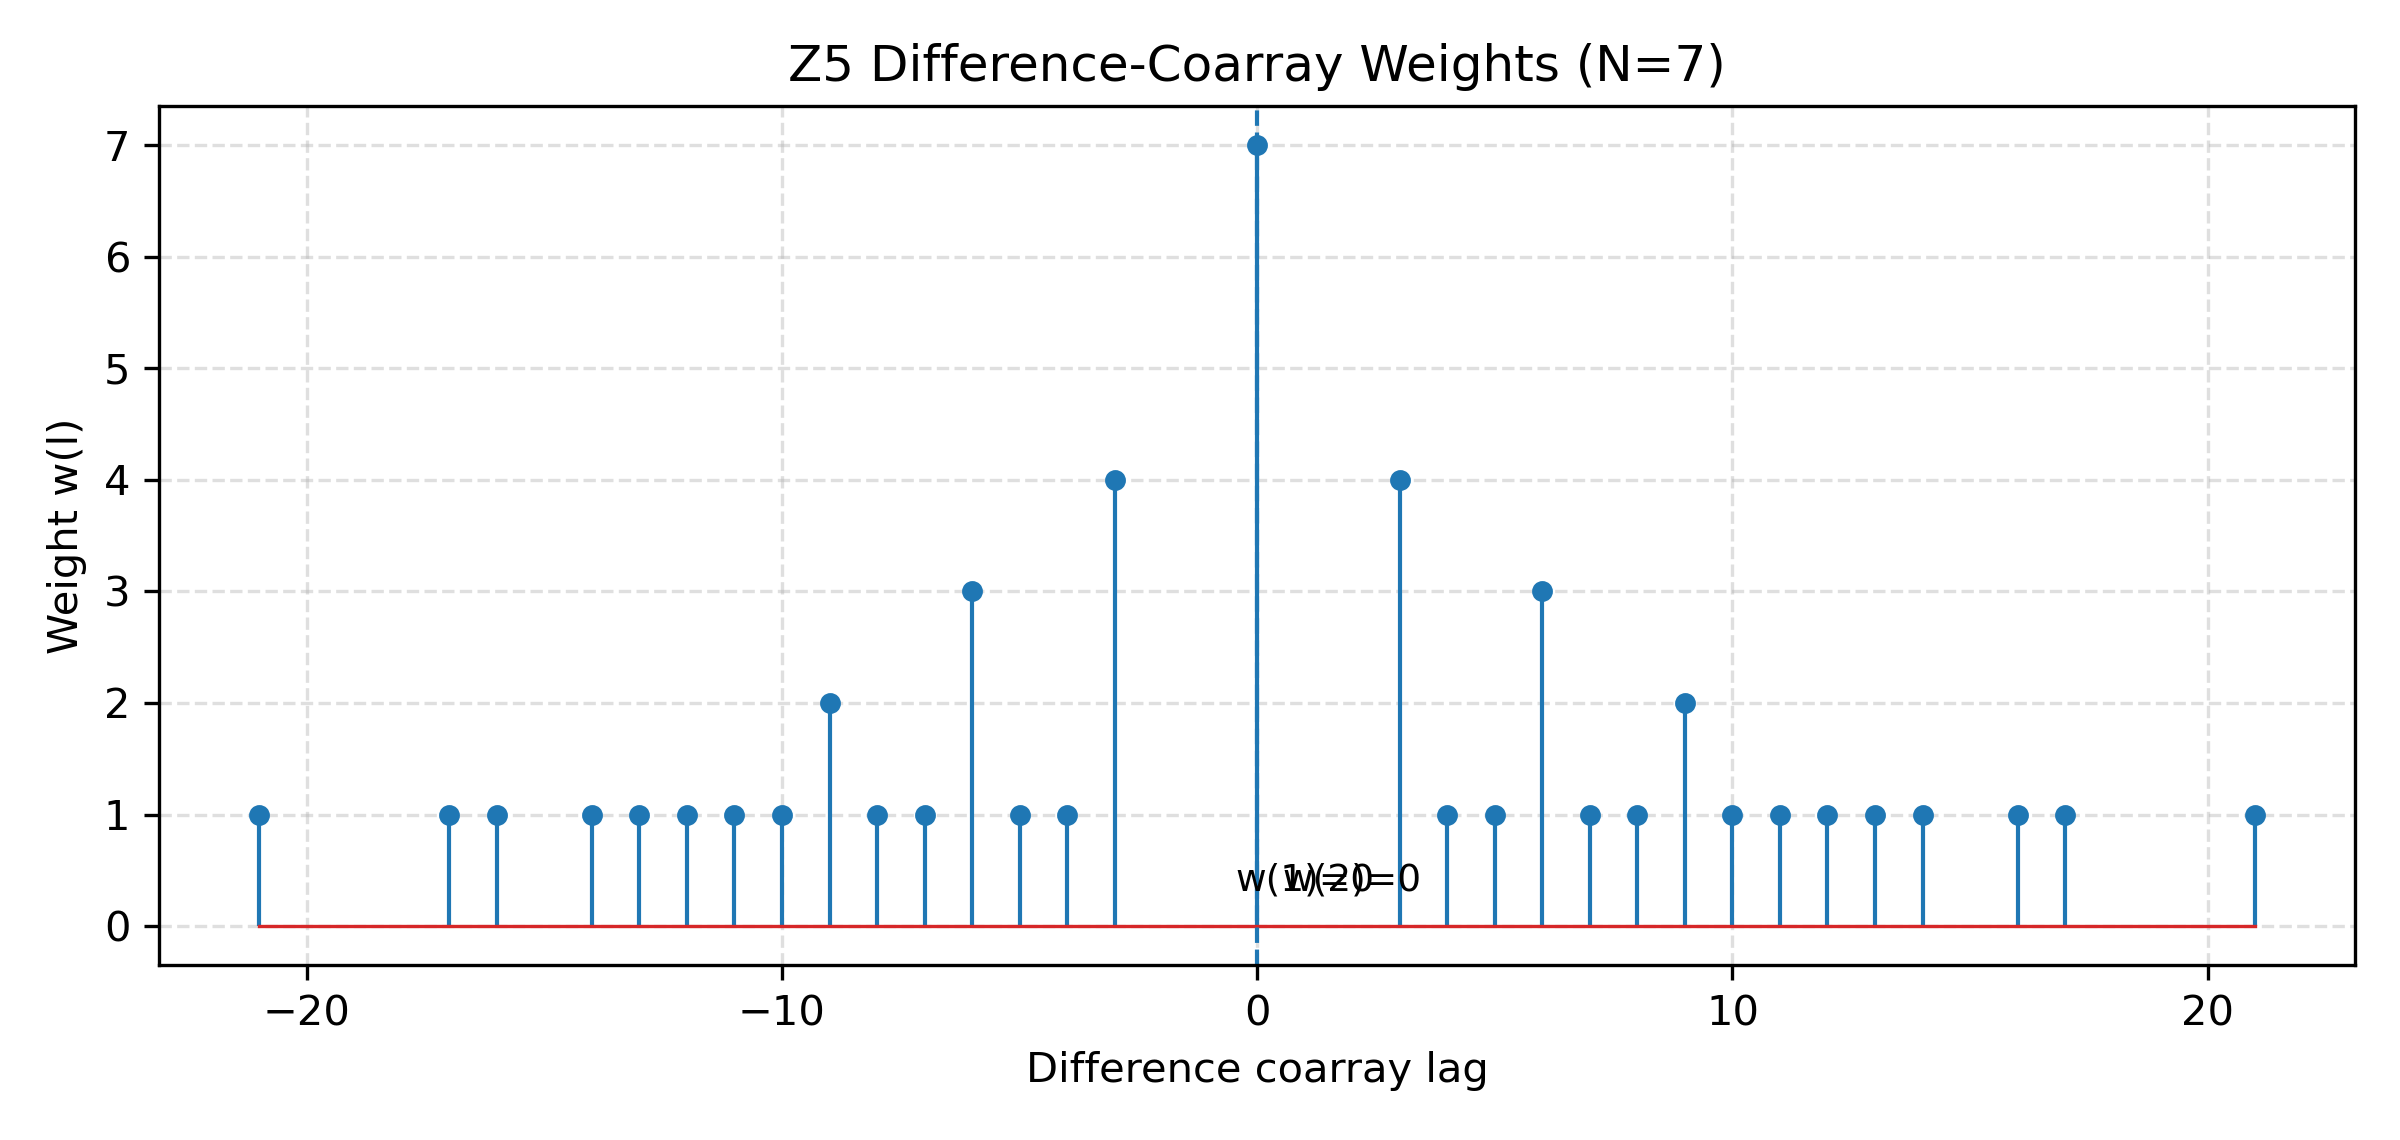
\includegraphics[width=\linewidth]{../../results/figures/paper1_conceptual/z5_coarray_weights.png}
\caption{Difference-coarray weight distribution of the canonical Z5 array. The missing critical small lags $w(1)=0$ and $w(2)=0$ reduce sensitivity to closely spaced sensor-pair coupling, while the uneven lag weights motivate finite-snapshot coarray regularization.}
\label{fig:z5_coarray_weights}
\end{figure}

\subsection{ALSS Configuration}

The fixed ALSS configuration used throughout the trial-1000 experiment is
\begin{equation}
\begin{aligned}
    \texttt{alss\_mode}  &= \texttt{ar1},\\
    \texttt{alss\_tau}   &= 0.25,\\
    \texttt{alss\_coreL} &= 3.
\end{aligned}
\end{equation}

These parameters are not tuned separately for each SNR, snapshot count, or coupling condition. This fixed-parameter design is intentionally conservative because the goal is to test whether one selected ALSS configuration gives stable improvement across the reported Scenario 3 sweep.

\subsection{Coupling Conditions}

Two coupling conditions are evaluated:
\begin{itemize}
    \item $c_1=0.0$: no mutual coupling,
    \item $c_1=0.3$: mutual coupling enabled.
\end{itemize}
The no-coupling case provides a baseline for finite-snapshot behavior, while the coupled case tests whether ALSS remains beneficial when the array output is also affected by mutual coupling. The coupling experiment is used for estimator-level performance comparison; ALSS is not presented as an antenna-pattern correction or as an explicit mutual-coupling matrix estimator.

\subsection{Monte Carlo Trials and Sweeps}

Each reported condition uses 1000 Monte Carlo trials. The Scenario 3 sweep contains two parts. First, an SNR sweep is performed at a fixed snapshot count of $M=64$ using
\begin{equation}
    \mathrm{SNR} \in \{-5,\;0,\;5,\;10,\;15\}\ \mathrm{dB}.
\end{equation}
Second, a snapshot-count sweep is performed at fixed $\mathrm{SNR}=5$ dB using
\begin{equation}
    M \in \{32,\;64,\;128\}.
\end{equation}
Both sweeps are repeated for $c_1=0.0$ and $c_1=0.3$. Because the point $\mathrm{SNR}=5$ dB and $M=64$ belongs to both sweeps, the output contains 16 reported rows but 14 unique operating conditions.

The performance metric is DOA RMSE. Percentage improvement is computed by comparing the baseline Coarray MUSIC RMSE with the ALSS-enhanced Coarray MUSIC RMSE under the same operating condition.

\section{Results}

\subsection{Trial-1000 Numerical Summary}

Table~\ref{tab:trial1000_summary} summarizes the main trial-1000 result.

\begin{table}[!t]
\centering
\caption{Scenario 3 Z5 Trial-1000 Summary}
\label{tab:trial1000_summary}
\begin{tabular}{lcc}
\toprule
Metric & Reported Rows & Unique Conditions \\
\midrule
Rows / conditions & 16 & 14 \\
Mean improvement & 9.85\% & 9.76\% \\
Median improvement & 8.66\% & 7.73\% \\
Worst improvement & -0.50\% & -0.50\% \\
Best improvement & 33.79\% & 33.79\% \\
Positive cases & 15/16 & 13/14 \\
\bottomrule
\end{tabular}
\end{table}

The trial-1000 result confirms the trend observed in the earlier trial-500 validation. ALSS improves most reported cases, with positive improvement in 15 of 16 reported rows and 13 of 14 unique operating conditions. The worst case shows only a small degradation of $-0.50\%$, while the best case reaches $33.79\%$ improvement. This supports the interpretation that the selected ALSS configuration is generally beneficial for the tested Z5 Scenario 3 setting, but it also confirms that ALSS should not be described as universally harmless.

\subsection{Coupling-Level Comparison}

Table~\ref{tab:coupling_summary} compares the no-coupling and mutual-coupling cases.

\begin{table}[!t]
\centering
\caption{Coupling-Level Summary for Scenario 3 Z5 Trial-1000}
\label{tab:coupling_summary}
\begin{tabular}{lcc}
\toprule
Metric & $c_1=0.0$ & $c_1=0.3$ \\
\midrule
Interpretation & No coupling & Coupling enabled \\
Unique conditions & 7 & 7 \\
Mean improvement & 5.60\% & 13.92\% \\
Median improvement & 5.54\% & 11.47\% \\
Worst improvement & 0.91\% & -0.50\% \\
Best improvement & 10.98\% & 33.79\% \\
Positive cases & 7/7 & 6/7 \\
\bottomrule
\end{tabular}
\end{table}

The coupling-level comparison is the central numerical evidence of the paper. Without mutual coupling, ALSS improves all seven unique conditions with a mean improvement of $5.60\%$. With mutual coupling enabled, ALSS improves six of seven unique conditions and increases the mean improvement to $13.92\%$. This does not prove that ALSS compensates mutual coupling directly. Rather, it supports the more conservative interpretation that Z5 geometry and ALSS act through complementary mechanisms: the geometry reduces sensitivity to short-spacing coupling effects, while ALSS reduces finite-snapshot lag-estimation variance before virtual covariance reconstruction.

\subsection{Representative MUSIC Pseudospectrum}

Fig.~\ref{fig:music_pseudospectrum} provides an estimator-level view of the Scenario 3 Z5 behavior.
The figure compares a representative no-coupling baseline, a coupled baseline, and a coupled ALSS-enhanced Coarray MUSIC spectrum.
For this realization, the no-coupling baseline localizes the two sources at $-20^\circ$ and $15^\circ$.
Under mutual coupling, the baseline estimate exhibits a small peak-location shift near the positive-angle source.
After ALSS regularization, the estimated peak returns to the true $15^\circ$ location.

\begin{figure}[t]
\centering
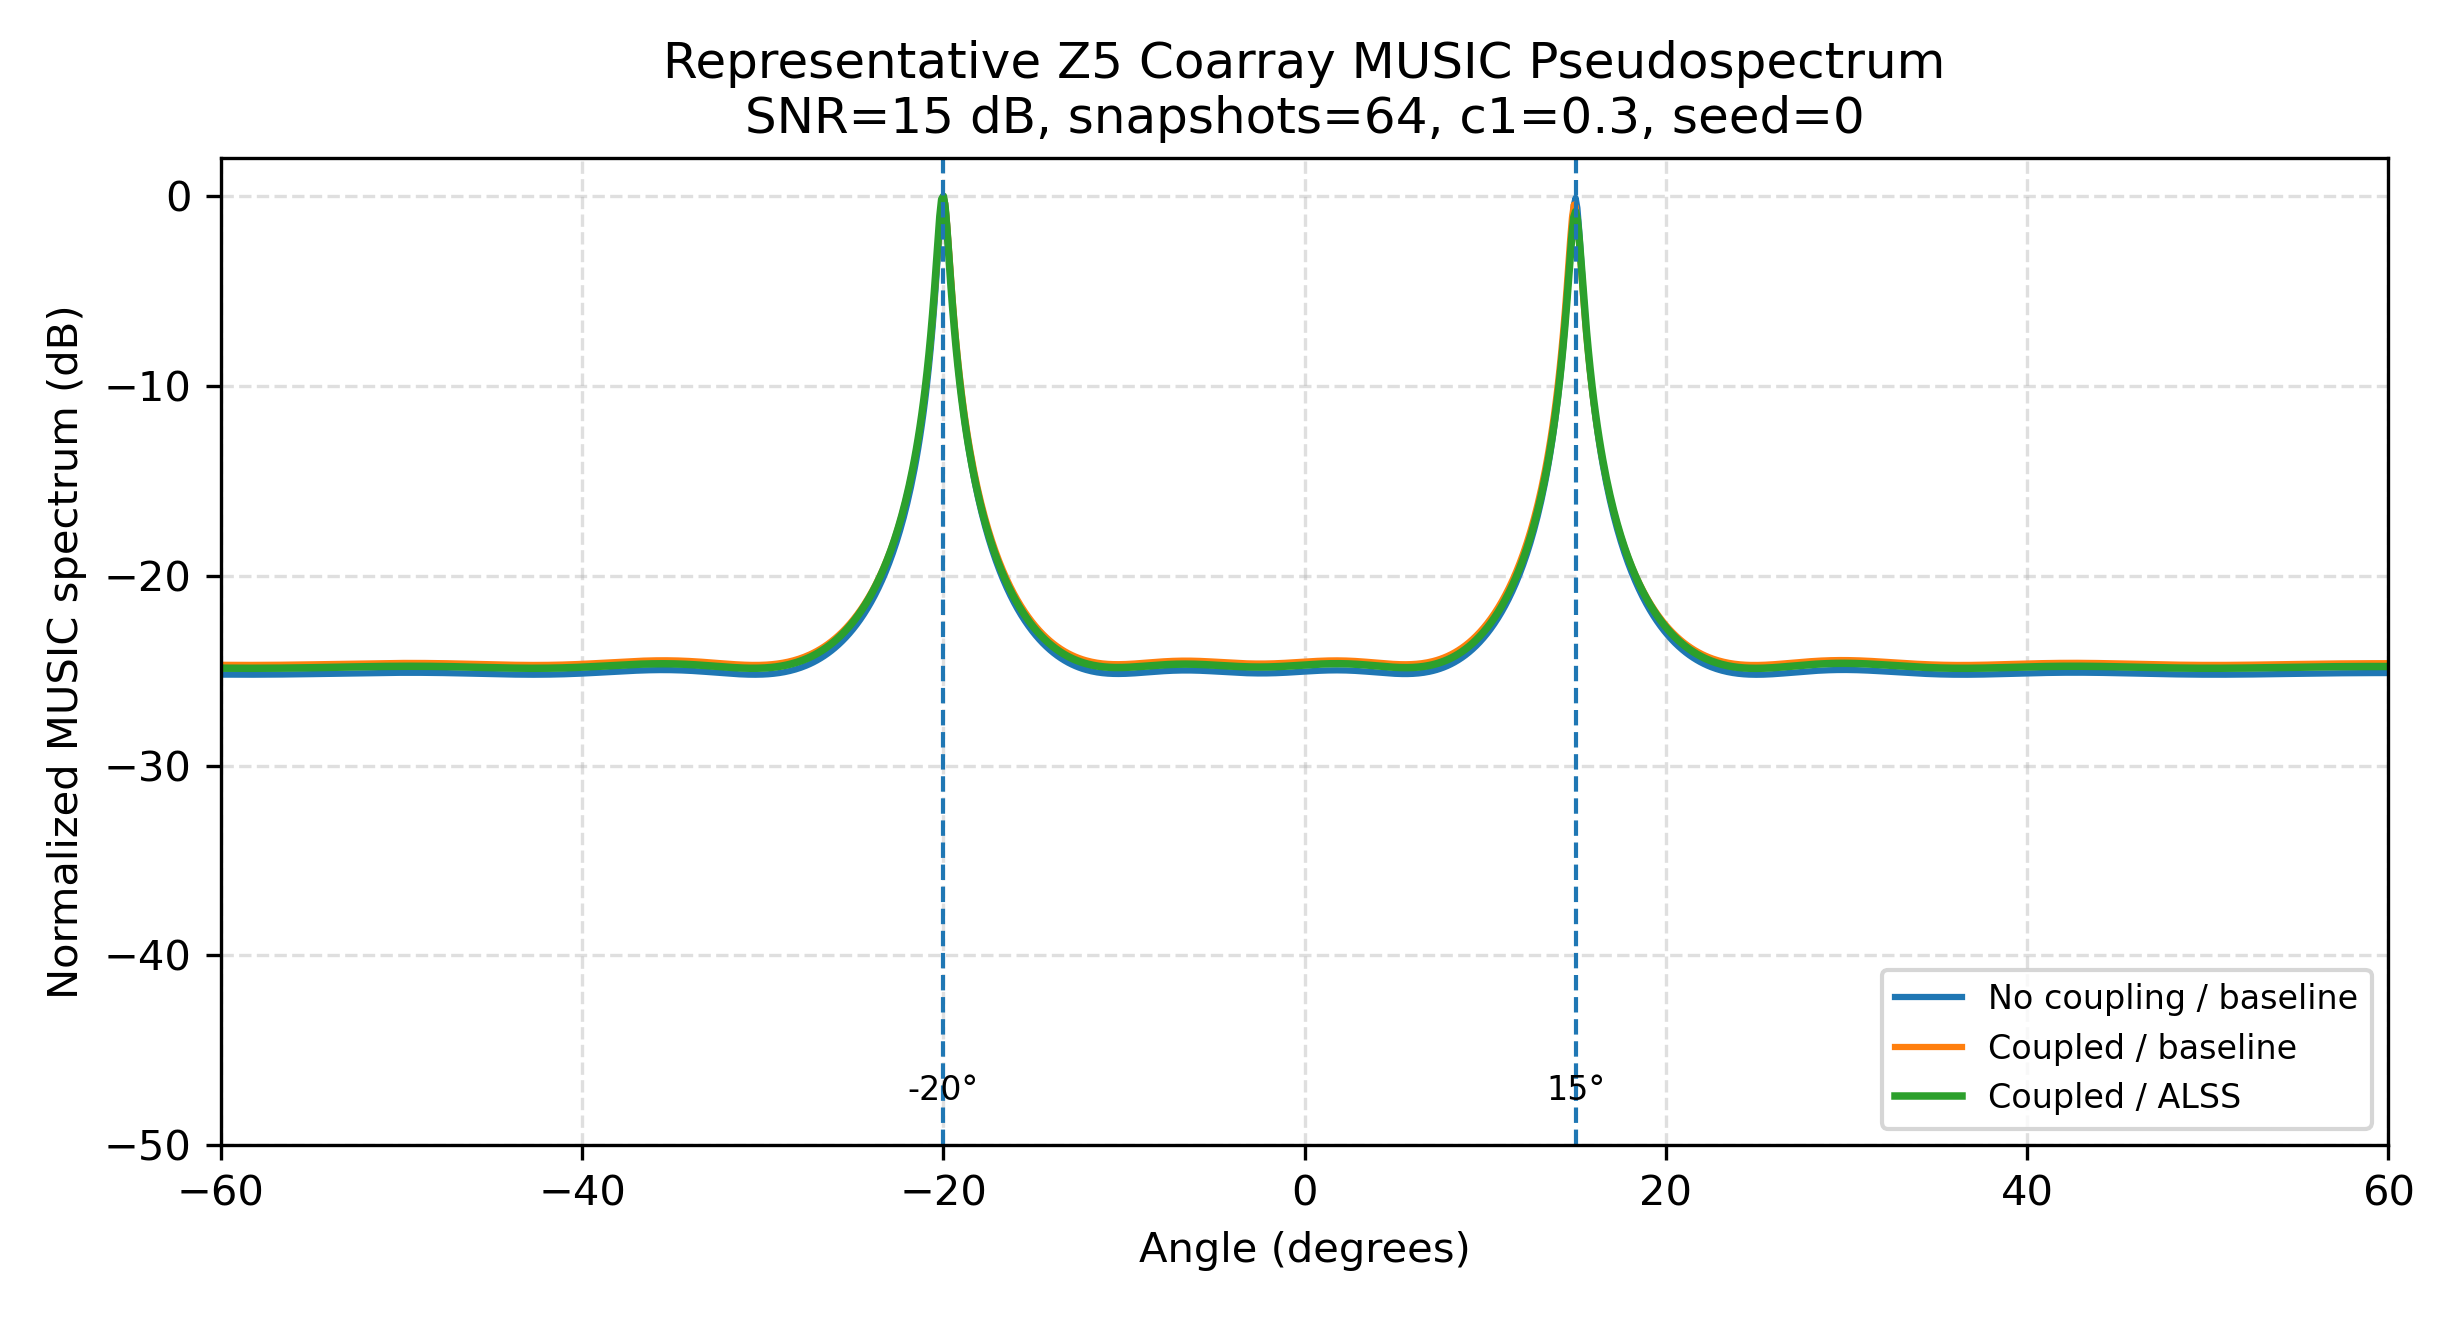
\includegraphics[width=\linewidth]{../../results/figures/paper1_conceptual/z5_music_pseudospectrum_comparison.png}
\caption{Representative Z5 Coarray MUSIC pseudospectrum comparison for no coupling, mutual coupling, and mutual coupling with ALSS. The example illustrates how ALSS regularization of coarray lag estimates can stabilize the MUSIC peak location in a coupled realization.}
\label{fig:music_pseudospectrum}
\end{figure}

This pseudospectrum is included as explanatory evidence, not as the primary statistical proof. A single realization cannot establish Monte Carlo performance. Its role is to connect the aggregate RMSE trends to the estimator mechanism: ALSS changes the coarray-domain correlation estimates used by the virtual covariance matrix, which can alter the MUSIC peak structure in a favorable way for some coupled realizations.

\subsection{Improvement Versus SNR}

Fig.~\ref{fig:improvement_snr} shows the percentage RMSE improvement versus SNR for both coupling conditions.

\begin{figure}[!t]
\centering
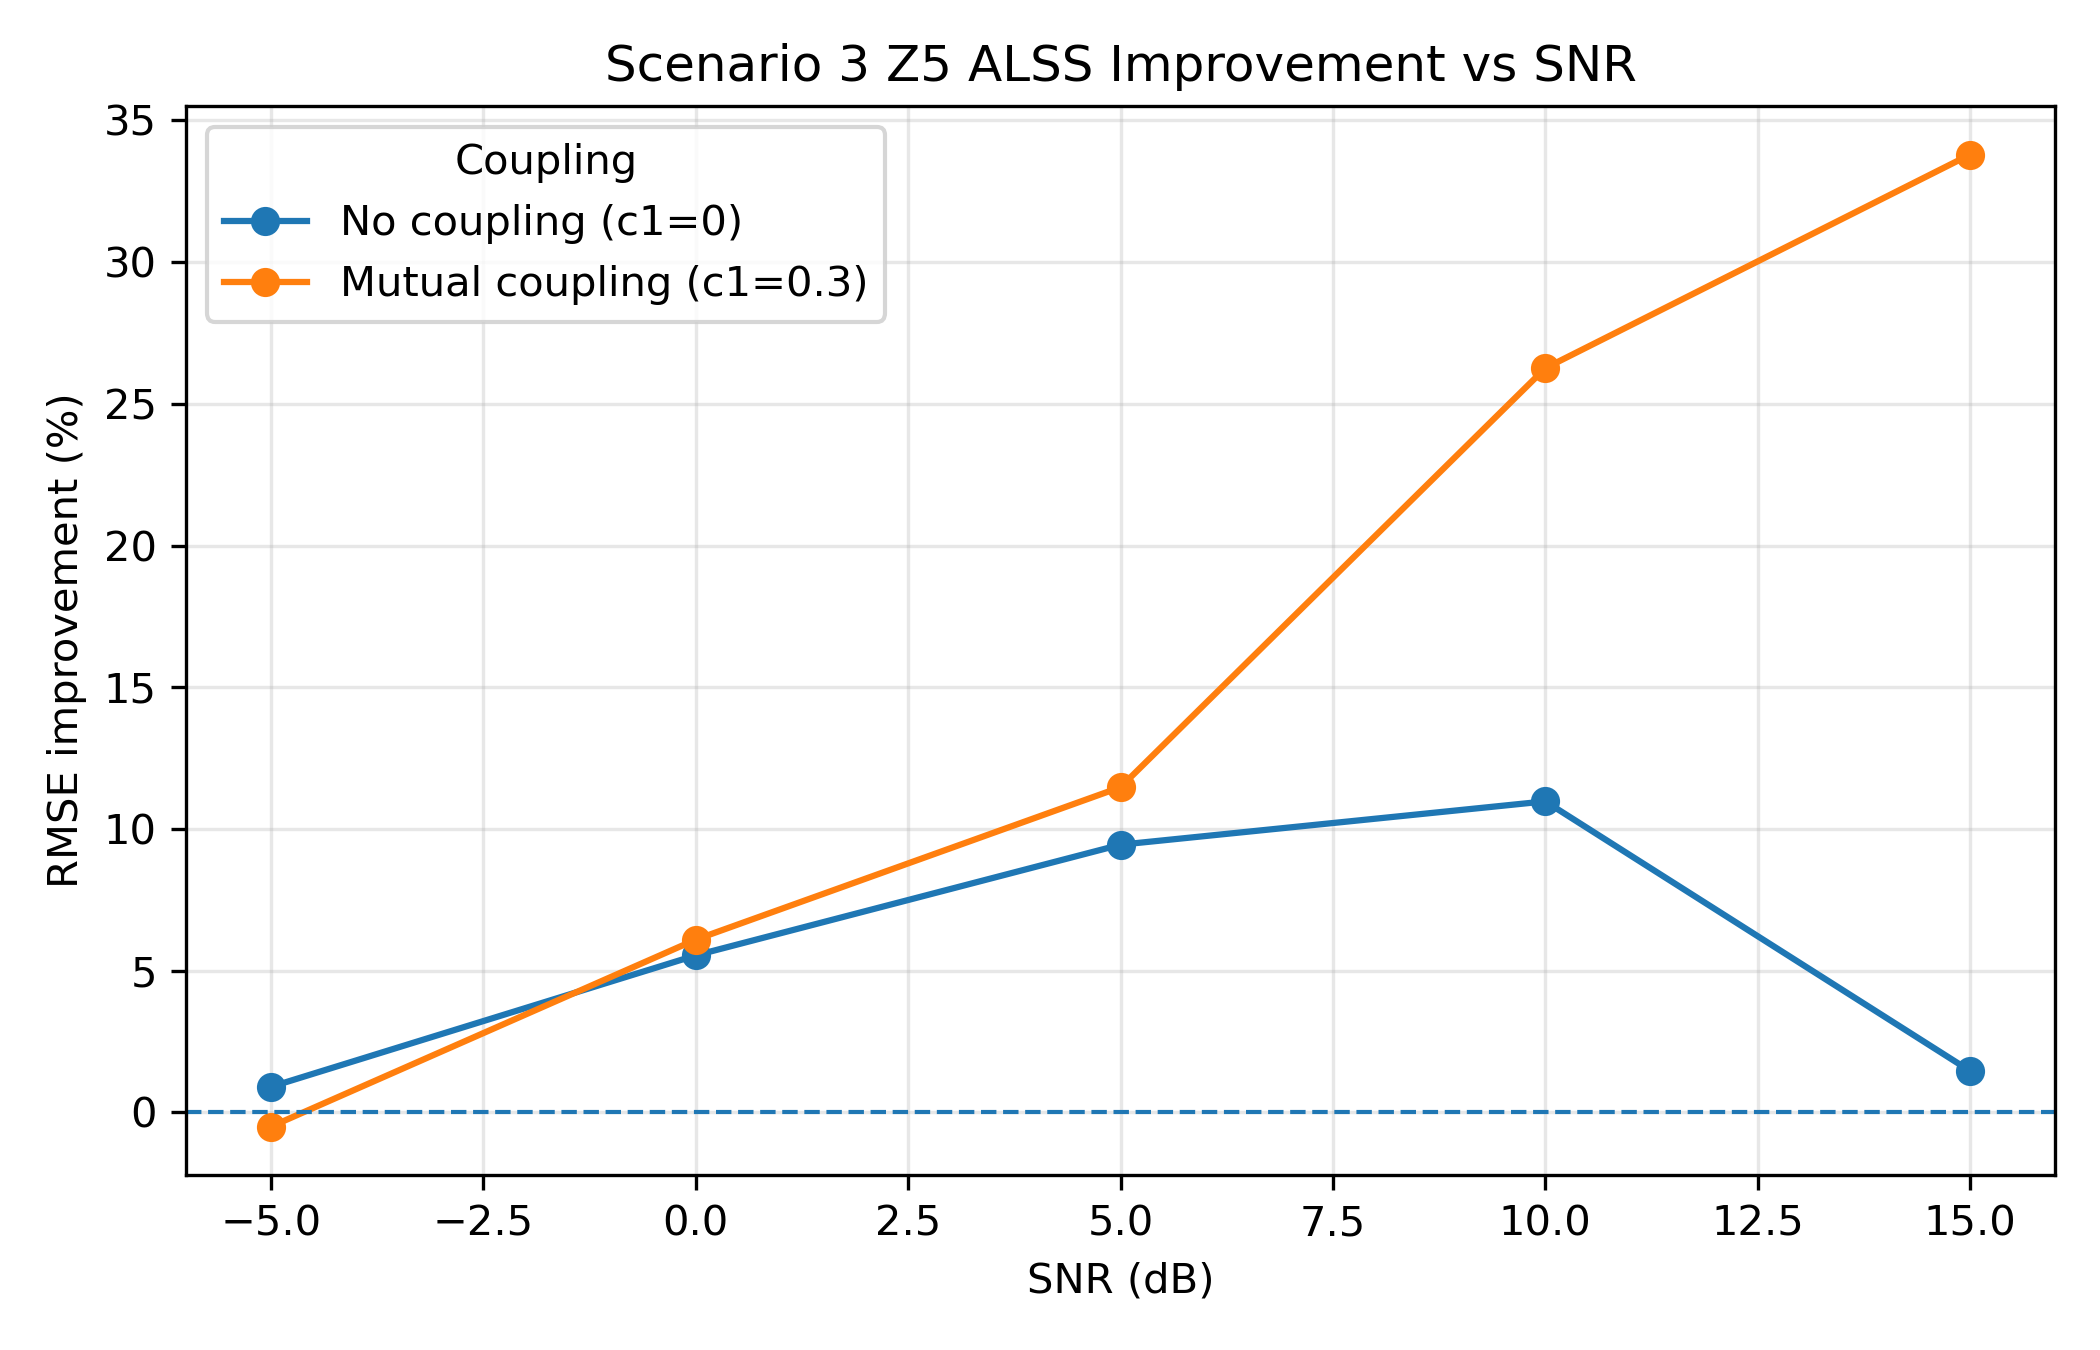
\includegraphics[width=\linewidth]{../../results/figures/scenario3_trial1000/scenario3_improvement_vs_snr.png}
\caption{Scenario 3 Z5 ALSS improvement versus SNR for no-coupling and mutual-coupling conditions.}
\label{fig:improvement_snr}
\end{figure}

The SNR sweep shows that ALSS improvement is consistently positive in the no-coupling case and generally stronger in the coupled case as SNR increases. At very low SNR, noise dominates the covariance estimate and limits the benefit of lag-selective regularization. At moderate-to-high SNR, the lag-estimation structure becomes more informative, and shrinkage of low-confidence lags produces larger relative gains, especially under mutual coupling.

\subsection{RMSE Under Mutual Coupling}

Fig.~\ref{fig:rmse_coupled} compares baseline and ALSS RMSE versus SNR when mutual coupling is enabled.

\begin{figure}[!t]
\centering
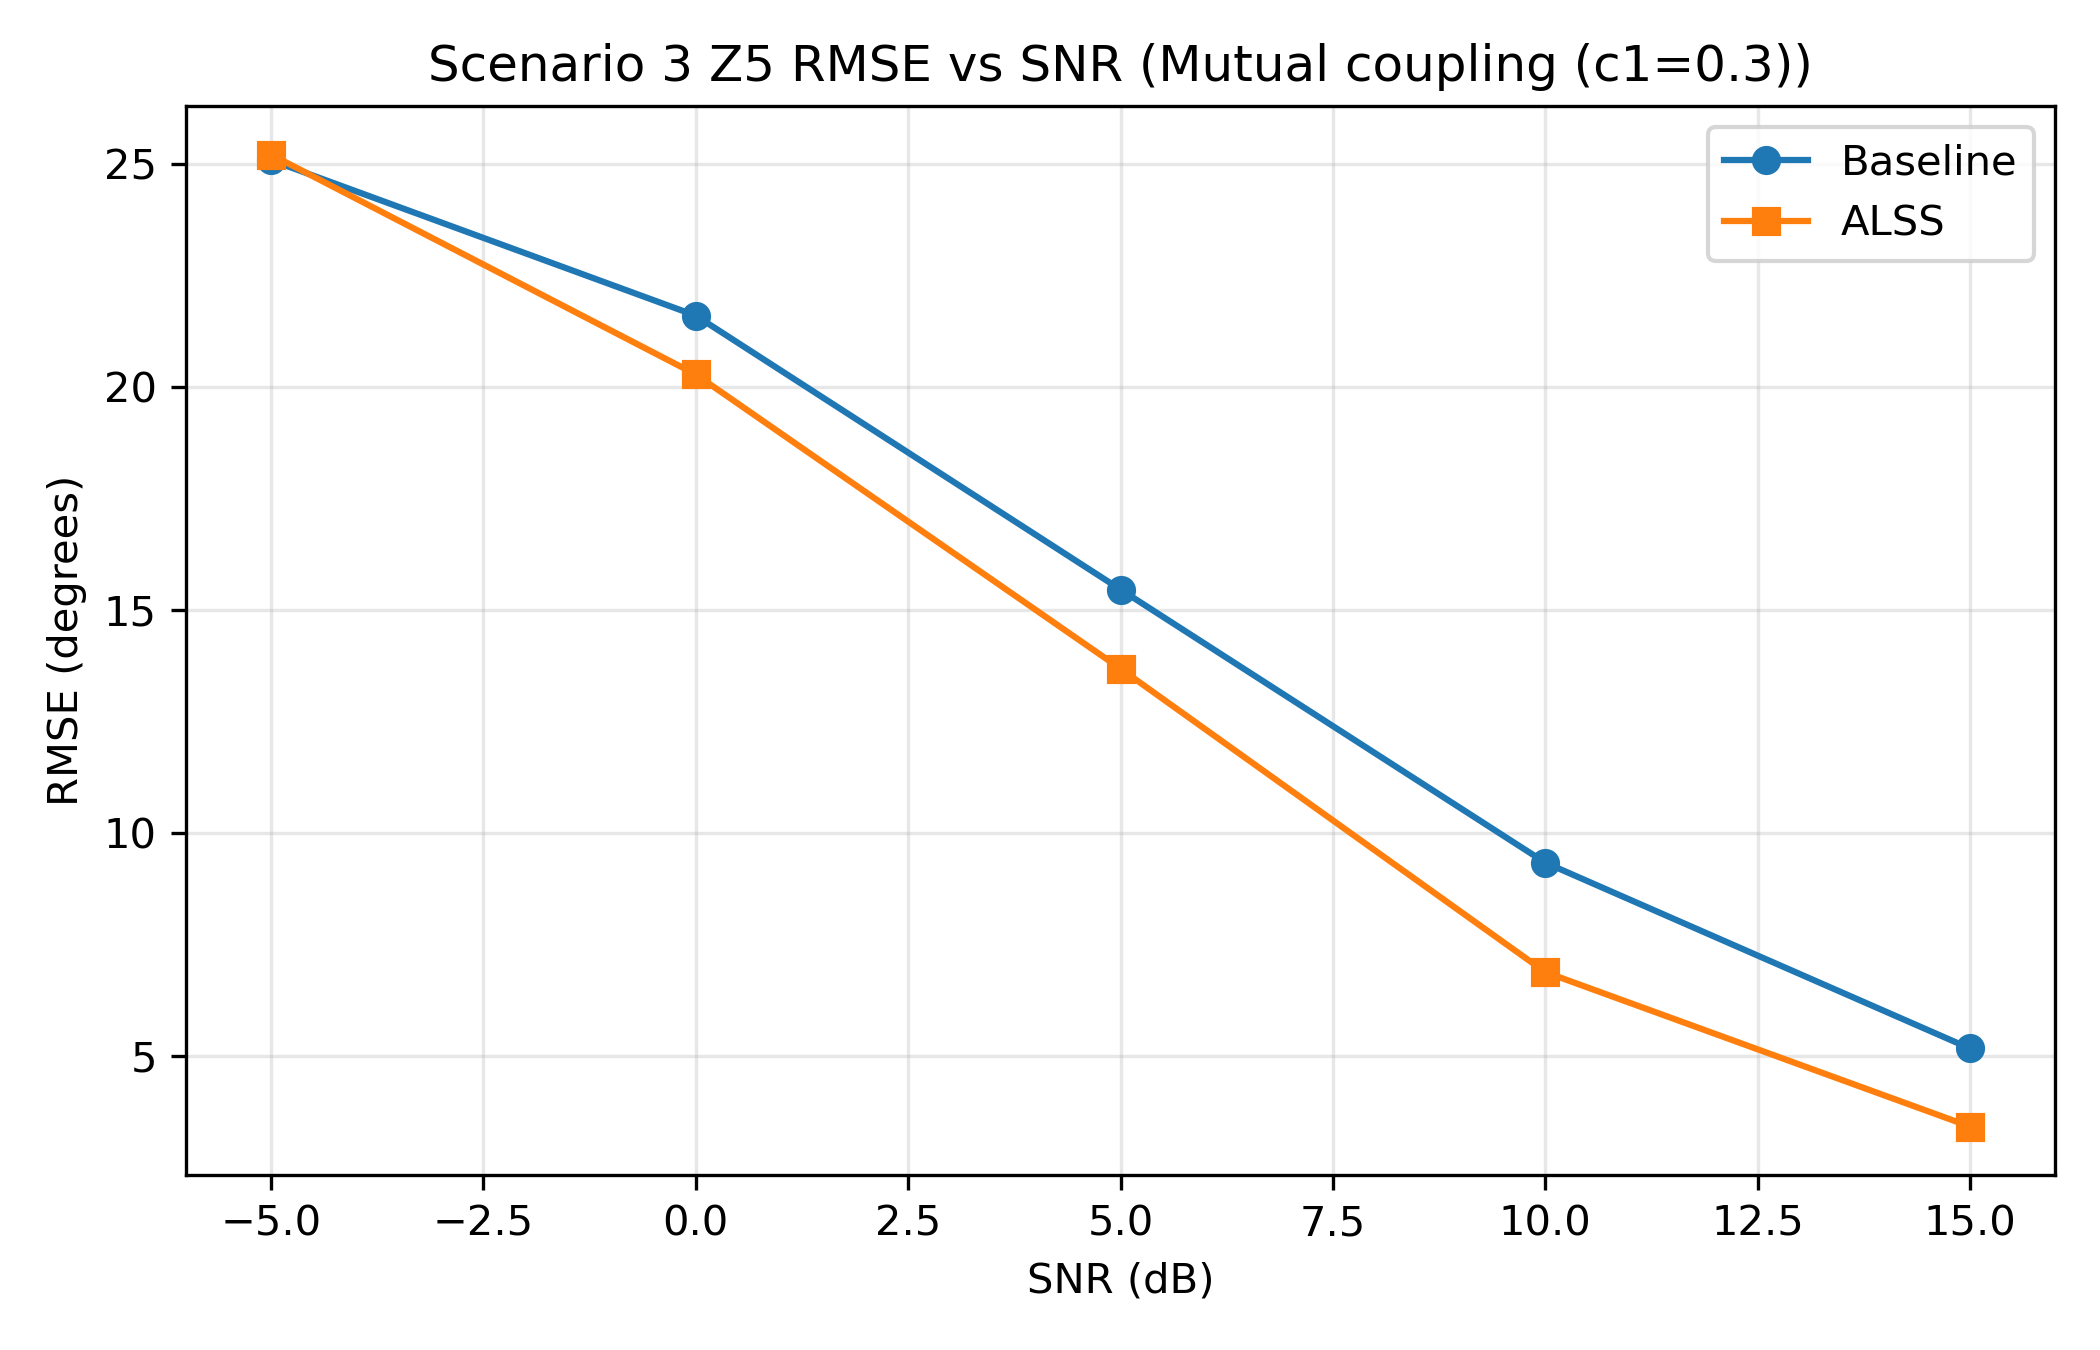
\includegraphics[width=\linewidth]{../../results/figures/scenario3_trial1000/scenario3_rmse_vs_snr_c1_0p3.png}
\caption{Scenario 3 Z5 RMSE versus SNR under mutual coupling ($c_1=0.3$).}
\label{fig:rmse_coupled}
\end{figure}

The coupled RMSE curve provides the most direct performance view for the challenging condition. ALSS reduces RMSE relative to baseline Coarray MUSIC for most tested SNR values under $c_1=0.3$. The reduction is most visible at moderate-to-high SNR, consistent with the improvement summary in Table~\ref{tab:coupling_summary}. The single weak case at the lowest SNR is consistent with the conservative conclusion that ALSS is beneficial in most, but not all, tested conditions.

\subsection{Improvement Versus Snapshots}

Fig.~\ref{fig:improvement_snapshots} shows the improvement versus snapshot count at fixed SNR $=5$ dB.

\begin{figure}[!t]
\centering
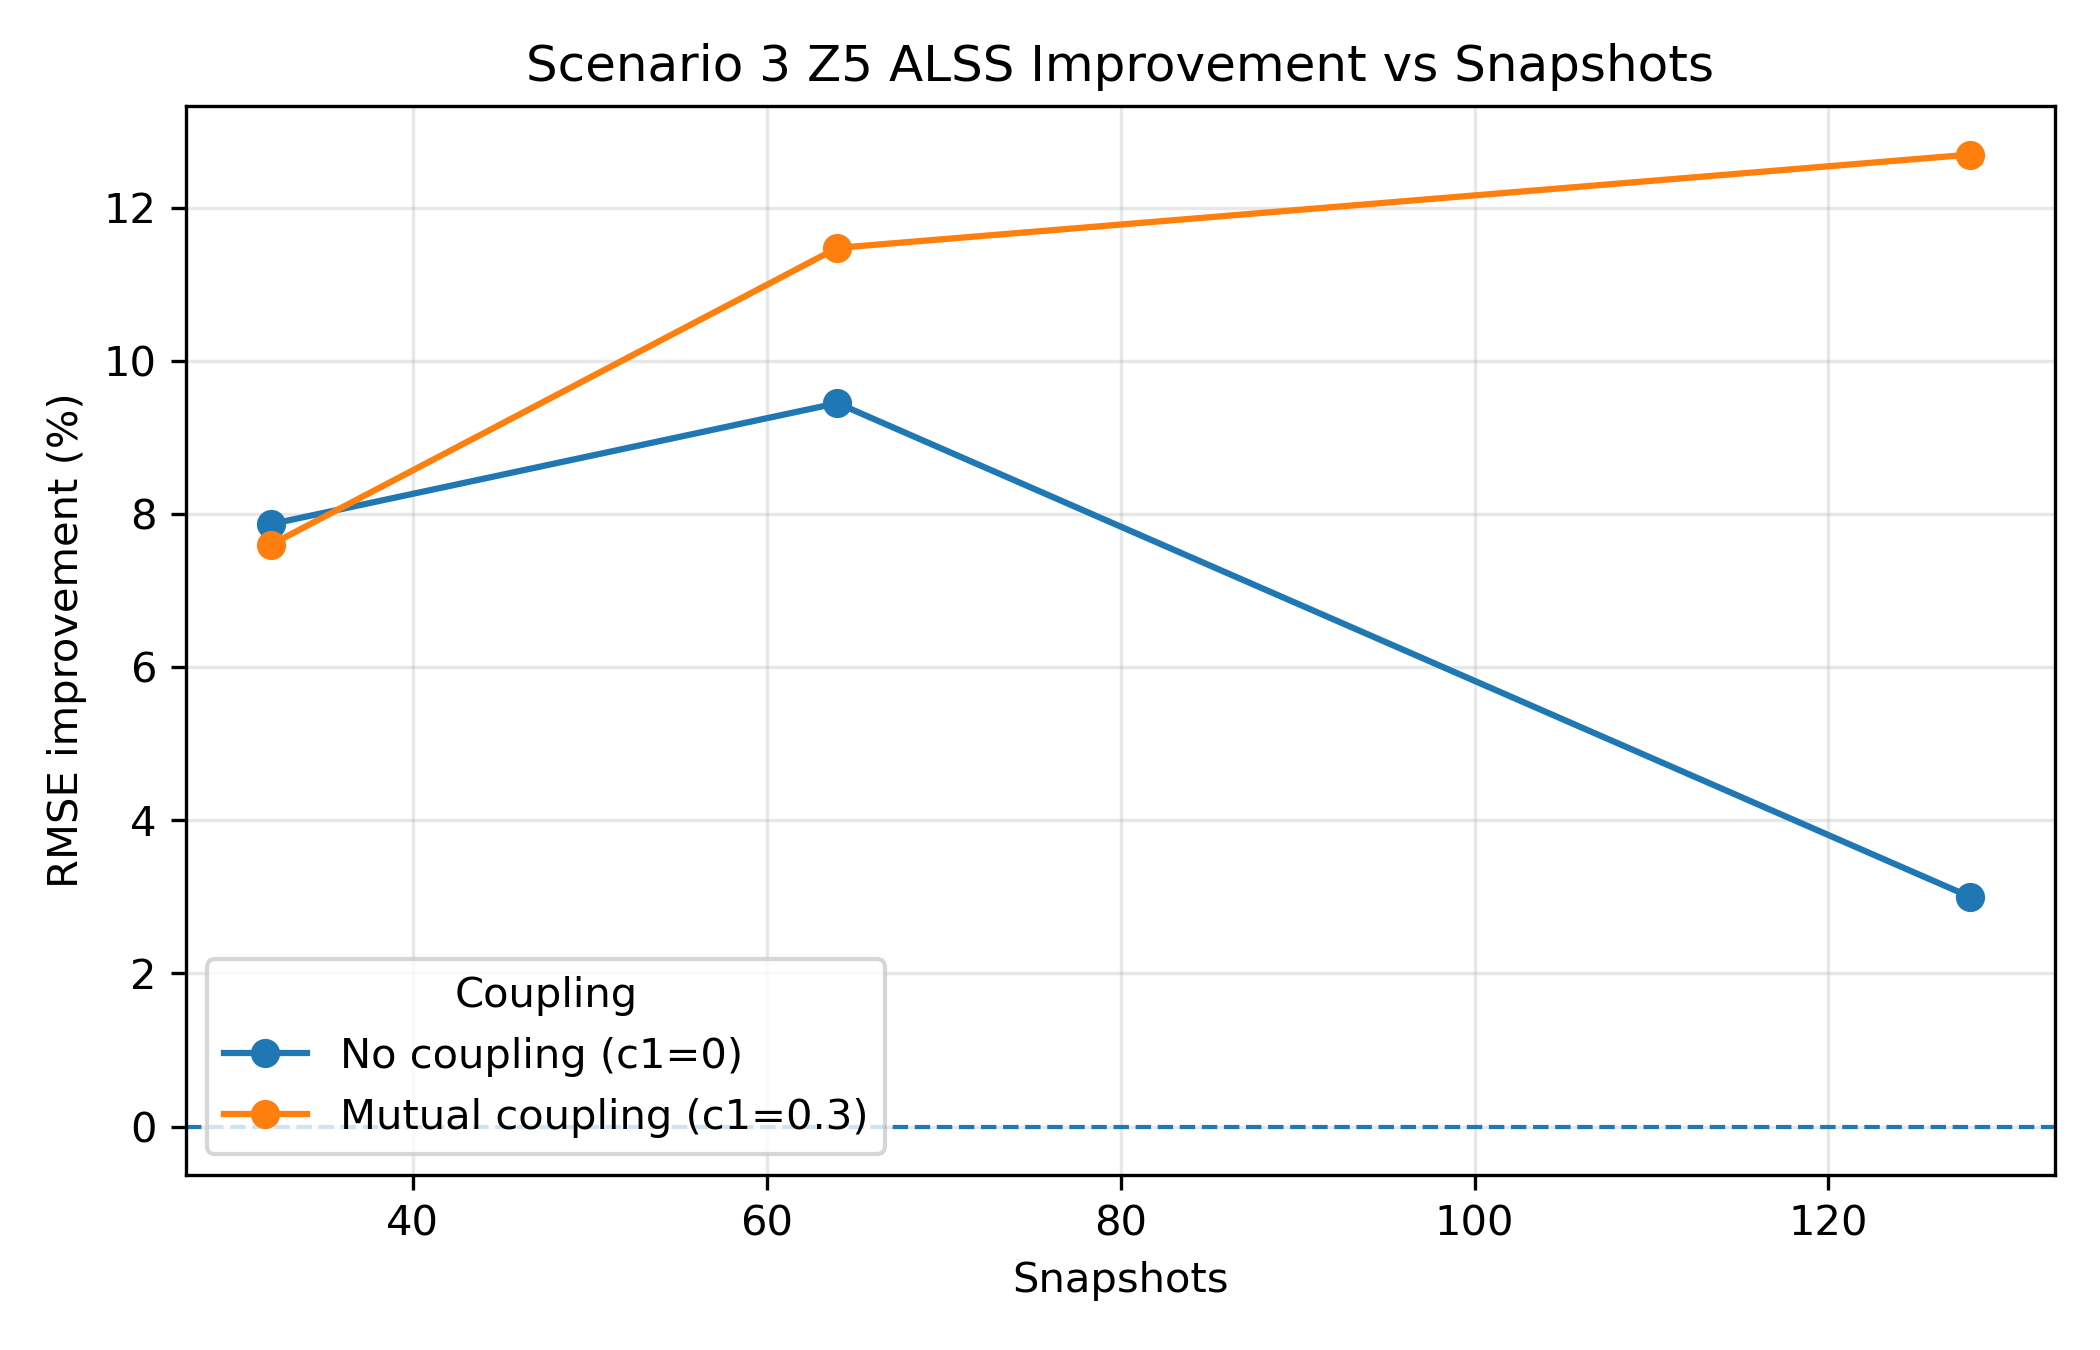
\includegraphics[width=\linewidth]{../../results/figures/scenario3_trial1000/scenario3_improvement_vs_snapshots.png}
\caption{Scenario 3 Z5 ALSS improvement versus snapshot count at fixed SNR $=5$ dB.}
\label{fig:improvement_snapshots}
\end{figure}

The snapshot sweep confirms that the selected ALSS configuration remains useful across the tested finite-snapshot range. The improvement remains positive for both $M=32$ and $M=128$, with the $M=64$ point appearing in both the SNR and snapshot sweeps. This supports the use of the trial-1000 result as the primary conference-paper evidence while leaving broader snapshot regimes for future validation.

\section{Discussion and Limitations}

The trial-1000 result supports a conservative claim: for the canonical Z5 sparse array under Scenario 3, ALSS with \texttt{ar1}, $\tau=0.25$, and $L_c=3$ improves Coarray MUSIC RMSE in most tested conditions. The improvement is stronger when mutual coupling is enabled, which supports the interpretation that geometry-level coupling robustness and post-geometry lag regularization can be complementary.

The role of Z5 is important in this interpretation. The array suppresses the most coupling-sensitive small lags, with $w(1)=0$ and $w(2)=0$, but its coarray-weight distribution is still uneven. Therefore, Z5 is a useful test case for the ALSS hypothesis: a geometry can be favorable for coupling robustness while still leaving finite-snapshot variance in low-confidence coarray lag estimates. ALSS targets this second effect.

This paper does not claim that ALSS changes the physical antenna pattern, modifies the sensor geometry, or directly estimates the mutual-coupling matrix. ALSS is applied only after sample covariance estimation and coarray lag averaging. Its effect is estimator-level: it regularizes the lag estimates used to form the virtual covariance matrix for Coarray MUSIC.

Several limitations remain. First, this paper is Z5-focused and does not yet establish performance across the full family of weight-constrained sparse arrays. Second, the MUSIC pseudospectrum example is representative and explanatory; it is not the primary statistical proof. Third, the mutual-coupling model is simulation-based and should not be interpreted as a complete electromagnetic antenna model. Fourth, only one fixed ALSS configuration is evaluated in the main trial-1000 result. A broader parameter-sensitivity study is required before making general tuning recommendations.

Future work should extend the validation to additional geometries such as Z1, Z3, Z4, and Z6, evaluate a wider range of SNR and snapshot regimes, and compare multiple ALSS parameter choices. A hardware-oriented extension is also natural because the processing chain contains FPGA-friendly kernels, including sample covariance formation, coarray lag averaging, virtual Toeplitz covariance reconstruction, and MUSIC spectrum scanning.

\section{Conclusion}

This paper presented a focused trial-1000 validation of Adaptive Lag-Selective Shrinkage for the canonical Z5 sparse array under Scenario 3 conditions. The results show that ALSS improves Coarray MUSIC RMSE in 15 of 16 reported rows and 13 of 14 unique operating conditions, with mean improvement of approximately $9.85\%$ over reported rows and $9.76\%$ over unique conditions.

The strongest observation is the coupling-dependent trend. Under no mutual coupling, ALSS achieves approximately $5.60\%$ mean improvement across unique conditions. Under mutual coupling with $c_1=0.3$, the mean improvement increases to approximately $13.92\%$. This supports the central interpretation of the paper: Z5 geometry reduces sensitivity to coupling-related short-spacing effects, while ALSS provides a complementary statistical regularization layer for finite-snapshot coarray lag estimates.

The paper does not claim universal ALSS optimality or full multi-geometry validation. Instead, it establishes a compact and reproducible Z5-focused conference result. Future work will extend the study to additional weight-constrained sparse arrays, evaluate ALSS parameter sensitivity, and investigate hardware-friendly acceleration of the covariance and coarray-processing pipeline using FPGA/HLS methods.
\bibliographystyle{IEEEtran}
\bibliography{references}

\end{document}